% SVN info for this file
%!TEX root = report.tex
\svnidlong
{$HeadURL$}
{$LastChangedDate$}
{$LastChangedRevision$}
{$LastChangedBy$}

\begin{abstract}

\begin{figure}[ht!]
\centering
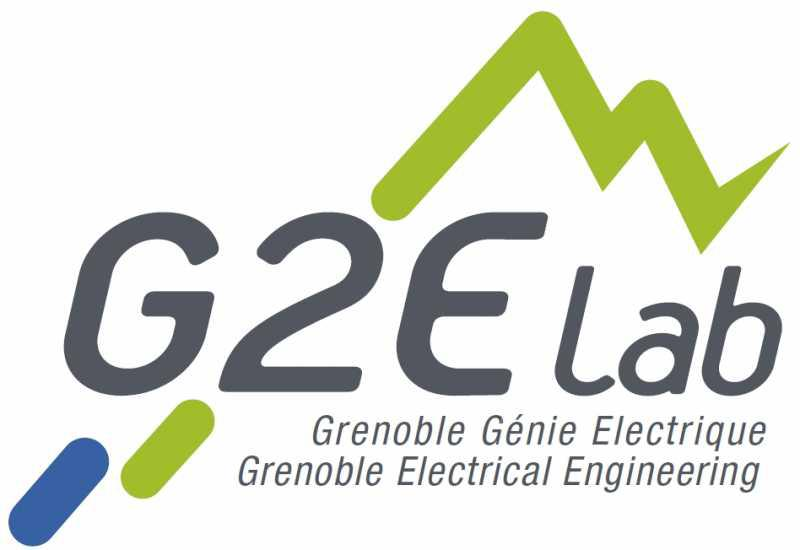
\includegraphics[width=30mm]{Logos/g2elab_logo.jpg}
\end{figure}
\par\vspace{5ex}

The research work leading to this thesis was carried out in the Grenoble Electrical Engineering Laboratory (G2E Lab) in the Grenoble Institute of Technology. The laboratory has several departments and teams working on varied research fields, including power electronics, magnetic materials, and microsystems. The team which carries out research in Electrical Power Systems is called SYREL (\textit{Syst\`{e}mes et R\'{e}seaux ELectriques}).\\

SYREL is the largest team in France that deals with Electrical Power Systems. Its core competencies encompass the entire electricity chain: from generation through transmission and distribution, till end-user consumption. The team focuses on the development, optimization and control of power systems, and works on many aspects and future technologies in this domain, while considering several other aspects like the economy, ecology and quality of energy.\\

There are three main axes in which research is carried out at SYREL:\\
\begin{itemize}
\item Non-conventional Connected Systems
\item Advanced Analysis and Optimization of Power Systems and
\item Advanced methods for Understanding and Securing Complex Infrastructures
\end{itemize}
\par\vspace{3ex}

The Non-conventional connected systems group deals with the control of non-conventional sources/sinks of energy connected to power networks, like renewable energies, electric vehicles etc., The second axis deals with the optimization of power systems, particularly distribution networks, and proposes methods to exploit flexibilities in these networks, forecast consumption using smart meters etc., The third axis deals with the issues like protection of large power systems, fault identification and localization and intelligent distribution. The research work done is in the second axis of research, concerning the management of the effect of integration of renewable energies into distribution networks.\\

More information about the SYREL team (in French, PDF only) is available \href{http://www.g2elab.grenoble-inp.fr/recherche/l-equipe-systemes-et-reseaux-electriques-217211.kjsp?RH=G2ELAB_R-SYREL}{{\color[rgb]{0.01,0.42,0.83} here}}.

\end{abstract}
